\vspace{-0.1cm}
\section{Retrying by Registration}
\label{sec:reg}
\vspace{-0.2cm}



%%SL.06.12: I think at least part of the motivation (maybe here or in the previous section) should include some discussion of how, in MPC, we can solve longer-horizon tasks by having a reasonable cost function that causes even a short-horizon planner to make steady progress toward the goal. From here, we can motivate that simply trying to match the image pixels of the target image is not a good cost, and part of the issue with long-horizon tasks via video prediction is really in the cost function. Prior work {ours} addresses this by using the motion predicted by the model to estimate positions of designated pixels (i.e., points on an object of interest) and measure their distance to the destination. But this requires tracking the object, and it's easy to lose track of the object during a complex manipulation where it might become occluded. In this work, we instead aim to estimate distances between images, registering the current image to the goal and using this registration to evaluate a distance. We will demonstrate in Section~\ref{something} that this substantially improves the performance of control via video-prediction, particularly on temporally extended tasks.

%Motivation for registering pixels
While self-supervision enables training powerful models to predict raw sensor inputs (among other quantities), using these model for control (e.g., with model-predictive control) poses the challenge of defining an appropriate cost function. One na\"{i}ve approach of formulating a cost function for video-prediction based control could be using the pixel-wise error between a \emph{goal image} and the predicted image. Goal images have the advantage that they are very general and do not make any domain specific assumptions. Minimizing this pixel-difference cost with respect to the action sequence passed into the model should result in a controller that tries to bring the system into the goal state. However there are a number of issues with this approach: first when objects in the image are far from the position in the goal image (e.g., they do not overlap) there is no gradient signal of the pixel-difference cost with respect to the actions. Second, due to the blurry predictions obtained from video-prediction model, the pixel-wise difference between the predictions and the goal image can become meaningless. Another possible approach would be to perform a registration between predicted video frames and the goal-image and using the average length of the warping vectors as a cost function for ``closeness" to the goal image; however, registering blurry prediction to a sharp goal-image poses a similar challenge as before. Another major drawback of cost functions based on metrics computed on the complete image is that they naturally ``pay attention'' to large objects in the image (such as the arm) whereas small objects only contribute negligible amounts to the costs. As a result the planner only tries to match the positions of the big objects (mainly the arm) ignoring smaller objects.

The main contribution of this work is a method for computing the planning cost based on image-to-image registration, which yields distances between a user-defined tracked object and its target location in the start- or goal-image. As a result, the cost is well-shaped, allowing for efficient optimization.

\begin{wrapfigure}{r}{.5\columnwidth}
\vspace{-0.25in}
\centering
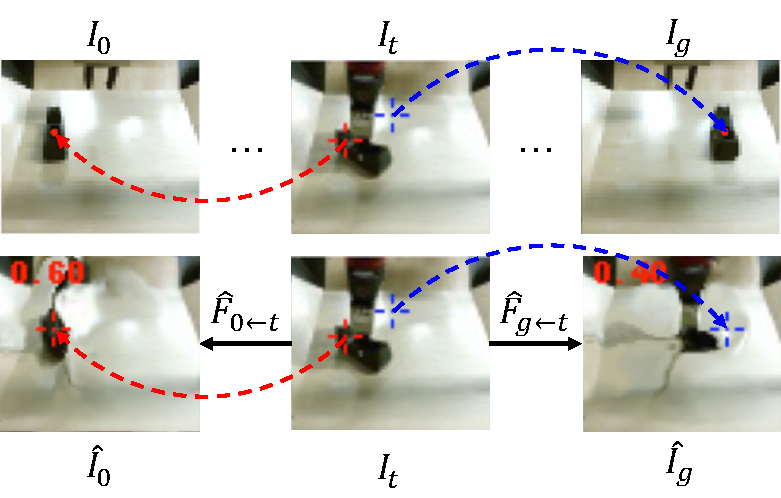
\includegraphics[width=0.5\columnwidth]{images/registration_singletime.pdf}
% \vspace{-0.1in}
\caption{\small{Closed loop control is achieved by registering the current image $I_t$ globally to the first frame $I_0$ and the goal image $I_g$. In this example registration to $I_0$ succeeds while registration to $I_g$ fails since the object in $I_g$ is too far away. \todo{replace with highres warping}}
\label{fig:reg_single}
\vspace{-0.2in}
}
\end{wrapfigure}


%%CF.06.15: the transition from the above to the below is rather abrupt.
\paragraph{Closed-loop video-prediction based control}

When the robot interacts with an object, the position of that object may change in unexpected ways, and therefore it is crucial that the system can update its belief of where the target object is. Prior work on visual MPC lacked this capability. To enable the agent to ``keep retrying" indefinitely until the task is accomplished we propose to use an image-to-image registration approach to find the target object in the current frame. 
We show that this tracking capability can be learned completely unsupervised from the data collected by the robot autonomously. As one might expect the self-supervised tracking approach works better for images that are closer to each other and sometimes fails when the entities in the image are too far apart. To increase accuracy and robustness in addition to the starting image our method can register to a goal-image. The goal image is optional and can be provided by a human or through demonstration.

\subsection{Test time procedure}

We will first describe the architecture at test time (see Figure~\ref{fig:registration_arch}(a)). The start and goal images $I_0$ and $I_g$ are passed into the registration network $R$ (implemented as a fully-convolutional neural network) which is trained to return flow maps $\hat{F}_{0 \leftarrow t} \in \mathbb{R}^{H \times W \times 2}$. The flow map is a vector field in $\mathbb{R}^2$ (with the same size as the image) which describes the relative motion for every pixel between two frames.
\begin{align}
    \hat{F}_{0 \leftarrow t} = R(I_t, I_0) &&
    \hat{F}_{g \leftarrow t} = R(I_t, I_g)
\end{align}

The flow map $\hat{F}_{0 \leftarrow t}$ can be used to warp the image of the current time step $t$ to the start image $I_0$, and $\hat{F}_{g \leftarrow t}$ can be used to warp from $I_t$ to $I_g$ (see Figure \ref{fig:reg_single} for an illustration):
\begin{align}
    \hat{I}_0 = \hat{F}_{0 \leftarrow t} \diamond  I_t &&
    \hat{I}_g = \hat{F}_{g \leftarrow t} \diamond  I_t 
\end{align}
Where $\diamond$ denotes a bilinear interpolation operator which interpolates the pixel value bilinearly with respect to a location $(x,y)$ and its four neighbouring pixels in the image.
In addition to start and goal images, the user needs to specify one or several designated pixel positions (for simplicity showing only the case for one designated pixel) $d_0 \in \mathbb{N}^2$ in the start image and the corresponding pixels locations $d_g \in \mathbb{N}^2$ in the goal image (the goal image is optional) to define the task. While the registration network is trained to perform a global registration between the images, we only evaluate it at the points $d_0$ and $d_g$ chosen by the user. Note that this results in a cost function that ignores distractors. For a current image $I_t$, $\hat{F}_{0 \leftarrow t}$ puts it in correspondence with $I_0$, and $\hat{F}_{g \leftarrow t}$ puts it in correspondence with $I_g$. The registration network is then used to find the pixel locations corresponding to $d_0$ and $d_g$ in the current frame: 
\begin{align}
    \hat{d}_{0,t} = d_0 + \hat{F}_{0 \leftarrow t}(d_0) &&
    \hat{d}_{g,t} = d_g + \hat{F}_{g \leftarrow t}(d_g)
    \label{eqn:warped_pos}
\end{align}

\begin{figure}[t!]
    \centering
    \begin{subfigure}[b]{0.25\textwidth}
        \centering
        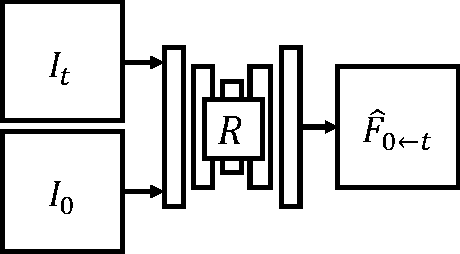
\includegraphics[width=\textwidth]{images/registration_test_start.pdf}\vspace{2.5mm}
        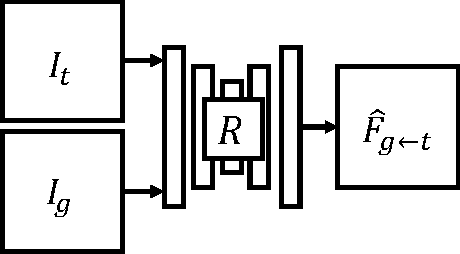
\includegraphics[width=\textwidth]{images/registration_test_goal.pdf}
        \caption{\small{Testing usage.}}
    \end{subfigure}
    \quad \quad
    \begin{subfigure}[b]{0.55\textwidth}
        \centering
        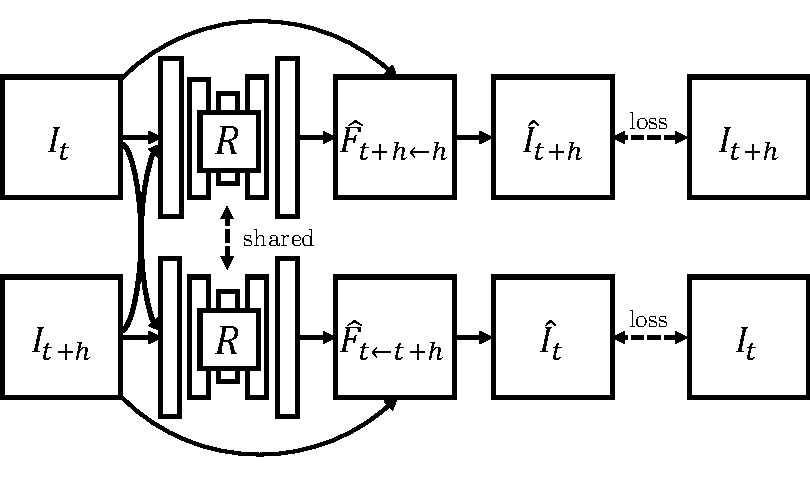
\includegraphics[width=\textwidth,trim={0 3mm 0 3mm},clip]{images/registration_train.pdf}
        \caption{\small{Training usage.}}
        \label{fig:discrete}
    \end{subfigure}
    \vspace{-1mm}
    \caption{\small{(a) At test time the registration network registers the current image $I_t$ to the start image $I_0$ (top) and goal image $I_g$ (bottom), inferring the flow-fields $\hat{F}_{0 \leftarrow t}$ and $\hat{F}_{g \leftarrow t}$. (b) The registration network is trained by warping images from randomly selected timesteps along a trajectory to each other.
    }}
    \label{fig:registration_arch}
\end{figure}

\begin{figure}
    \centering
    \vspace{-0.1in}
    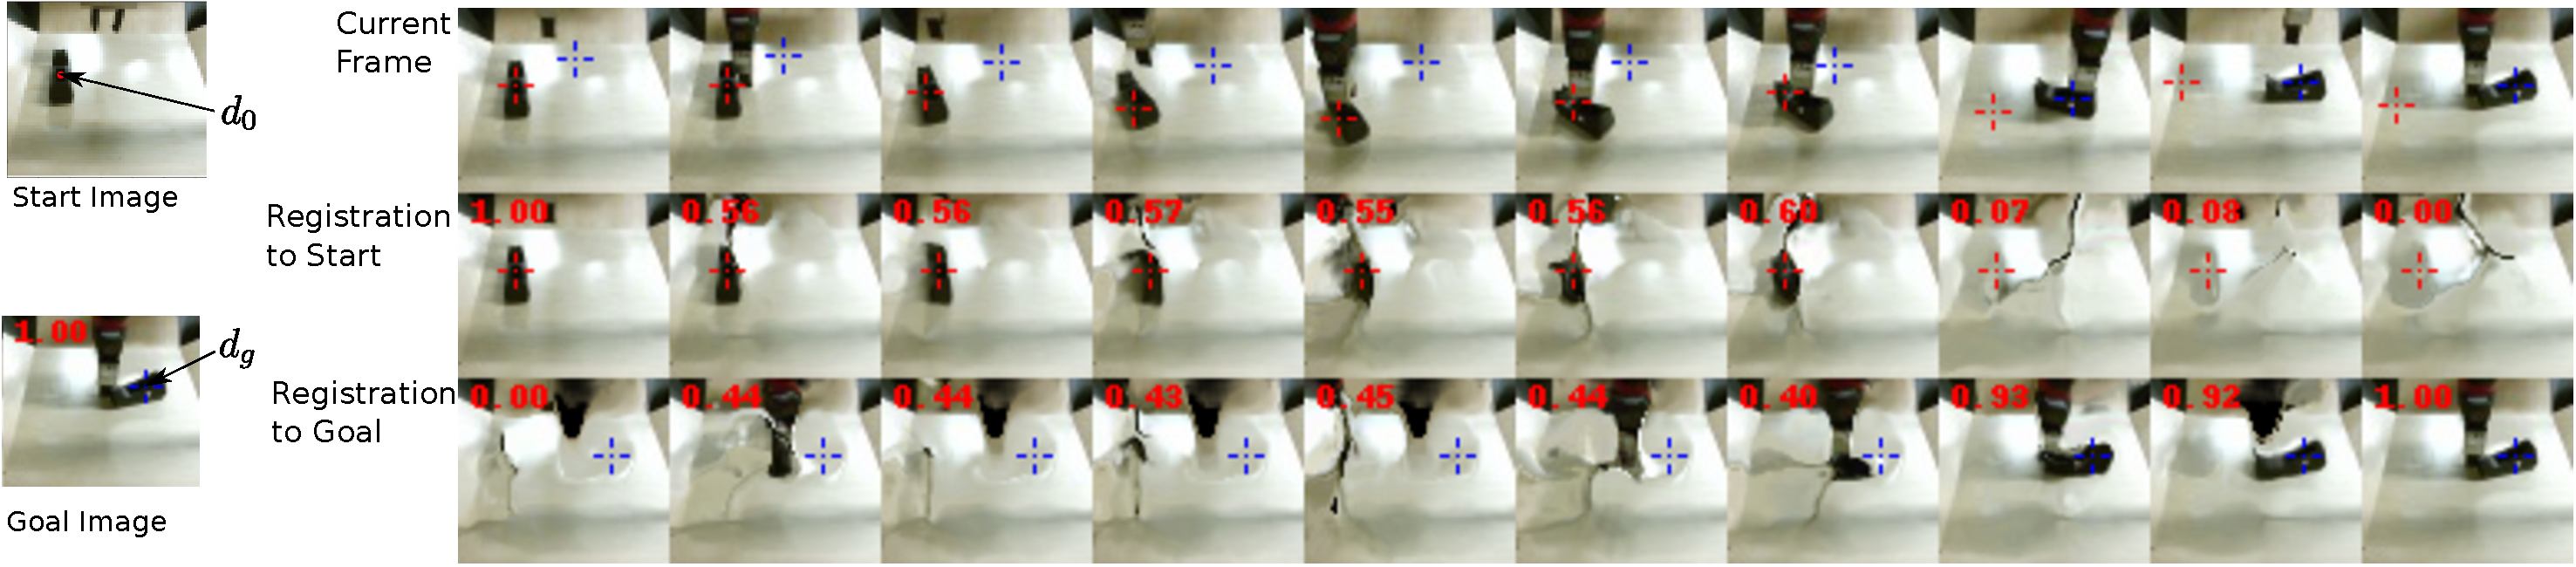
\includegraphics[width=1\textwidth]{images/registration_overtime.pdf}
    \caption{\small{Outputs of registration network. The first row shows images from a trajectory executed by the robot, the second shows each image warped to the initial image via registration, and the third shows the same for the goal image. A successful registration in this visualization would result in images that closely resemble the start (or goal). In these images, the locations where the designated pixel of the start image $d_0$ and the goal image $d_g$ are found is marked with red and blue crosses, respectively. It can be seen that, for the registration to the start image (red cross) the object is tracked for the first 6 frames, while the registration to the goal image (blue cross) succeeds for the last 3 time steps. The numbers in red (upper left corners) indicate the trade off factors $\lambda$ between the views and are used as weighting factors for the planning cost. (Best viewed in PDF)}}
    \label{fig:tracking_overtime}
    \vspace{-0.2in}
\end{figure}

In practice instead of a single flow vector we consider a neighborhood of flow-vectors around $d_0$ and $d_g$ and take the median separately in x and y direction making the registration more stable.
\autoref{fig:tracking_overtime} visualizes the tracking results during a pushing task. On the left we show the start image and goal image provided by the user at the beginning of the trajectory. The first row shows the video, with the estimated location of $d_0$ marked in red and the estimated location of $d_g$ marked in blue. In this example, registration succeeds with respect to the first image succeeds for the first 7 steps but fails after that (with successful registration we mean that the cross is on the object of interest). However registration with respect to the goal image succeeds for the last 3 steps. Thus, there is enough information at each time step to determine the cost, which we discuss in detail in the next section.

%%SL.06.12: Something to keep in mind here: When describing a learned model, often a good recipe is to first explain the model itself (which is what you're doing here), and then explain how that model is trained. It's important to stick to good abstraction. If the model implementation (i.e., the neural net) is complicated, it can help to first explain it abstractly, then explain the objective, and only then explain how it is instantiated in a neural network. Perhaps this organization can be adopted in this section.



%SL.06.12: I think we need a separate paragraph that discusses two views... this paragraph seems to mix together two different things

%%SL.06.12: for top-level organization, we should have separate subsections for registration and for control. Maybe a reasonable top-level organization I might suggest is:
% 3 Preliminaries
% 4 Overview (summarize how the method works and say what the parts are, so the sections that follow don't come as a surprise)
% 5 Retrying with Registration
% 5.1 Self-Supervised Registration of Goal and Source Images <- this would have \paragraphs for algorithm, training/objective, and model
% 5.2 Deriving Planning Costs from Self-Supervised Registration <- can mention designated pixels here
% 6 Task Setup and Implementation <- all the stuff about how the task is set up, action space, etc
% of course, other organizations are possible, but maybe this gives a hint for how to get started



